\documentclass{article}
\usepackage[margin=2cm]{geometry}
\usepackage{graphicx}
\usepackage[pages=some]{background}
\usepackage{titling}
\usepackage{tabularx}
\usepackage{tikz}
\usepackage{forest}
\usepackage{float}

\forestset{
  my box/.style={
    draw,
    rectangle,
    rounded corners,
    fill=gray!20,
    inner sep=6pt,
    minimum width=3cm % Adjust the width as needed
  }
}


\geometry{a4paper}

\backgroundsetup{
    scale=1,
    angle=0,
    opacity=1,
    contents={%
        
\includegraphics[width=\paperwidth,height=\paperheight]{institution_logo.jpg}
    }
}

\newcommand{\subtitle}[1]{
    \posttitle{
        \par\end{center}
        \begin{center}\large#1\end{center}
        \vskip0.5em}
}

\title{ME-463}
\author{Md. Hasibul Islam}
\subtitle{IC ENGINES}

\begin{document}
\begin{titlepage}
    \centering
    
    {\Huge\bfseries\maketitle}
    \textbf{Zahurul Haque Sir} \\
    \vspace{2cm}
    
\includegraphics[width=8cm]{institution_logo.jpg}
    \vfill
    \vspace*{2cm}
\end{titlepage}

\tableofcontents
\pagebreak
\section{Lecture 01: Introduction} 
\hfill Date: 04/06/2023

\section{Lecture 02: ENGINE FUELS} 
\hfill Date: 06/06/2023
\begin{itemize}
  \item In future → Diesel + 5-10\% bio-diesel
  \item In future → Petrol + Ethanol
  \item High H/C ratio indicates high value of energy \& heating
  \item Gasoline : 31,850 kJ/L 
  \item Average Human power in 0.2 hp, but an 1500 cc car has a power of 60 kW
  \item Octane number → Petrol Engines 
  \item Cetane number → Diesel Engines 
  \item High compression ratio → more knocking 
\end{itemize}

\subsubsection*{Octane Number}
The octane number is a rating used to measure the performance of gasoline (petrol) in spark-ignition engines. It indicates a fuel's resistance to knocking or detonation, which is the spontaneous combustion of the fuel-air mixture in the engine cylinder, causing a knocking sound. Knocking can lead to engine damage and reduced efficiency. The higher the octane number, the more resistant the fuel is to knocking.\\
Typically, two common octane rating methods are used: Research Octane Number (RON) and Motor Octane Number (MON). RON measures a fuel's performance under mild operating conditions, while MON evaluates it under more severe conditions. The octane number displayed at gas stations usually refers to the average of RON and MON, known as the Anti-Knock Index (AKI) or Pump Octane Number (PON).\\
Higher octane number is preferable. 


\subsubsection*{Cetane Number}
The cetane number is a rating used to measure the ignition quality of diesel fuel. It represents the fuel's ability to ignite quickly and burn efficiently in a compression-ignition (diesel) engine. Similar to the octane number, the cetane number is obtained through laboratory tests. It measures the delay between fuel injection and ignition in a diesel engine. Higher cetane numbers result in shorter ignition delays and more complete combustion.
\begin{itemize}
  \item It indicates the ability of self-ignite of engine.
  \item Higher cetane number may cause firing easily. 
  \item Lower cetane number creates knocking, and even create an explode of 2000°C.
  \item At lower cetane number, fuel will be mixed properly, because of time lagging. 
  \item Neither high cetane number, nor low cetane number is preferable. 
\end{itemize}

\subsubsection*{Why Octane number should be high, but cetane number should be in a specific range?}
While a higher octane number is generally preferable to resist knocking in spark-ignition engines, the ideal cetane number for diesel fuel is not too high or too low. Here's why:
\begin{itemize}
  \item \textbf{Too High Cetane Number}: If the cetane number of diesel fuel is excessively high, it can lead to a phenomenon known as "cetane number related ignition delay." This means the fuel ignites too quickly during the compression stroke, causing a rapid rise in pressure. This can result in increased engine noise, rough combustion, and potentially higher emissions.
  \item \textbf{Too Low Cetane Number}: On the other hand, if the cetane number is too low, the fuel may have a longer ignition delay, causing a delayed start of combustion in the diesel engine. This can lead to difficult cold-starting, rough idling, reduced engine performance, and increased emissions.
\end{itemize}

To achieve optimal performance, diesel fuels are typically formulated to have cetane numbers within a specified range that balances ignition quality, combustion efficiency, and emissions control. The specific range may vary depending on engine design, regional fuel standards, and operating conditions.It's important to note that the cetane number requirements may differ for different diesel engines and applications. For instance, high-performance engines or heavy-duty diesel engines may have different cetane number recommendations compared to standard passenger vehicle diesel engines. By maintaining an appropriate cetane number range for diesel fuel, it ensures proper ignition characteristics, smooth combustion, good cold-starting performance, improved fuel efficiency, and reduced emissions in diesel engines.

\begin{figure}
  \centering
  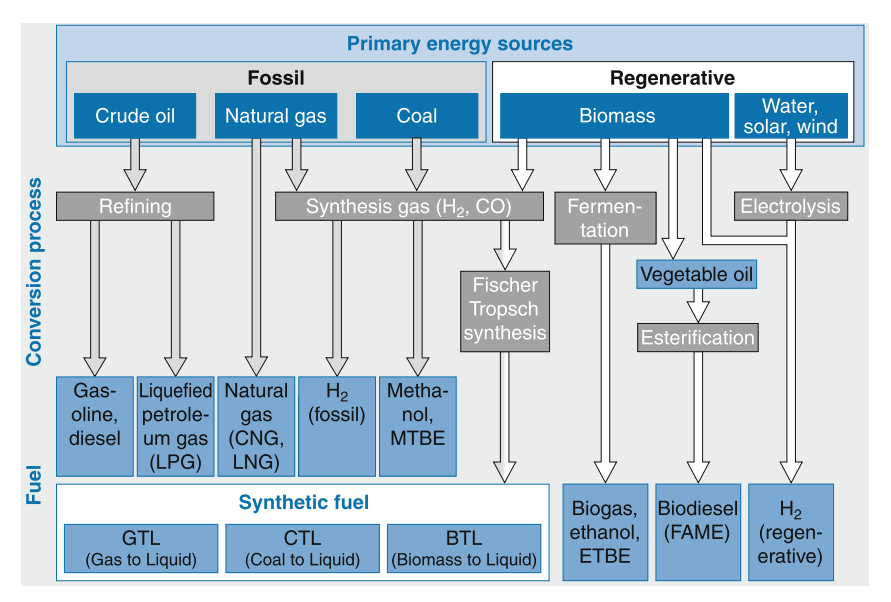
\includegraphics[width=0.95\textwidth]{img/energy.png}
  \caption{Primary Energy Sources.}
  \label{fig:Primary Energy Sources }
\end{figure}

\subsubsection*{Compression Ratio}
Compression ratio is a fundamental parameter used to describe the internal combustion process in an engine. It represents the ratio of the total cylinder volume when the piston is at the bottom of its stroke (bottom dead center) to the volume when the piston is at the top of its stroke (top dead center). In simpler terms, it quantifies how much the air-fuel mixture is compressed in the engine cylinder.\\

The compression ratio affects engine performance and efficiency in several ways, including its relationship with knocking:
\begin{itemize}
  \item Engine Power: A higher compression ratio generally leads to increased engine power output. This is because a greater compression ratio allows for more efficient combustion, resulting in better utilization of the fuel's energy.
  \item Engine Efficiency: A higher compression ratio can improve engine efficiency by extracting more energy from the fuel-air mixture. This is achieved through increased thermal efficiency, where more of the heat energy released during combustion is converted into useful work.
  \item Knocking: Knocking, also known as detonation, is an undesirable phenomenon where the air-fuel mixture in the cylinder detonates spontaneously before the spark plug ignites it. Knocking causes a knocking sound and can lead to engine damage if it occurs excessively.

\end{itemize}

The compression ratio has a significant impact on the likelihood of knocking. A higher compression ratio increases the cylinder pressure and temperature during compression, making the air-fuel mixture more prone to auto-ignition. If the fuel's octane rating is not high enough to resist knocking under the increased pressure and temperature, knocking can occur. The more compression ratio, the more knocking will happen.

To mitigate knocking, it is essential to use fuels with higher octane numbers in engines with higher compression ratios. Fuels with higher octane ratings have increased resistance to knocking, allowing them to withstand the higher pressures and temperatures associated with higher compression ratios.

\subsubsection*{H//C ratio}
The hydrogen-to-carbon ratio (H/C ratio) is a measure of the relative abundance of hydrogen and carbon atoms in a fuel molecule. It is commonly used to characterize the composition and properties of various fuels. The H/C ratio affects the energy content, combustion efficiency, and emission characteristics of a fuel.

\begin{figure}
  \centering
  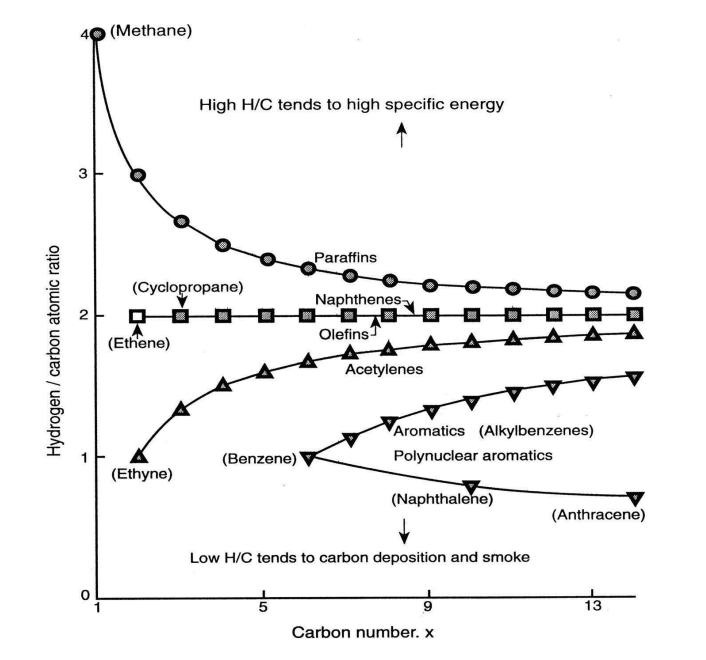
\includegraphics[width=0.75\textwidth]{img/hc_ratio.png}
  \caption{H:C atomic ratio of various inorganic hydrocarbon compounds.}
  \label{fig:Different H/C ratio }
\end{figure}

In general, fuels with higher H/C ratios tend to have higher energy content, as hydrogen has a higher energy content per unit mass compared to carbon. Fuels with higher H/C ratios also tend to burn more cleanly, producing fewer carbon dioxide (CO2) emissions and less particulate matter during combustion.


\subsubsection*{Diesel Fuel Specifications}
The terms 1-D, 2-D, and 4-D are commonly used to classify different grades or types of diesel fuel. These classifications are based on the volatility and viscosity characteristics of the fuel, and they are often associated with specific applications. Here's an overview of each type and their uses:

\begin{itemize}
  \item 1-D Diesel Fuel:
    \begin{itemize}
      \item 1-D diesel fuel is a lighter grade of diesel fuel that has a lower viscosity and higher volatility compared to 2-D and 4-D fuels.
      \item It is commonly used in colder climates or during winter months, as it has better cold flow properties and can prevent wax crystal formation at lower temperatures.
      \item 1-D fuel is often referred to as "winter diesel" or "arctic diesel" and is designed to perform well in low-temperature conditions.
      \item It is commonly used in applications such as transportation, agriculture, construction, and mining equipment operating in cold regions.
    \end{itemize}
  \item 2-D Diesel Fuel:
      \begin{itemize}
        \item 2-D diesel fuel is a mid-range grade of diesel fuel that has a moderate viscosity and volatility.
        \item It is suitable for use in a wide range of diesel engines and is the most commonly available type of diesel fuel in most areas.
        \item 2-D fuel is used in various applications, including passenger vehicles, trucks, buses, generators, boats, and industrial machinery.
        \item It is also used in heating systems, as it can be burned in oil furnaces or boilers for space heating.
      \end{itemize}

  \item 4-D Diesel Fuel:
      \begin{itemize}
        \item 4-D diesel fuel is a heavier grade of diesel fuel with a higher viscosity and lower volatility compared to 1-D and 2-D fuels.
        \item It is primarily used in industrial applications and heavy-duty engines that require more robust fuel properties.
        \item 4-D fuel is commonly used in large marine engines, locomotives, power generation, and industrial equipment.
        \item It may also be used in off-road vehicles and machinery, such as construction equipment and agricultural machinery.
      \end{itemize}

\end{itemize}

\subsubsection*{Automotive Fuels}
Automotive fuels are the types of fuels used to power vehicles, specifically designed for use in internal combustion engines found in cars, motorcycles, trucks, and other vehicles. The two primary types of automotive fuels are gasoline and diesel fuel.

\textbf{Gasoline}: Gasoline, also known as petrol, is a volatile fuel primarily used in spark-ignition engines. It is a mixture of hydrocarbons derived from crude oil through refining processes. Gasoline is designed to combust in spark-ignition engines, where a spark from the spark plug ignites the fuel-air mixture, generating power.

\textbf{Diesel Fuel}: Diesel fuel is a heavier and less volatile fuel used in compression-ignition engines, commonly known as diesel engines. It contains higher energy content compared to gasoline and is ignited through compression rather than a spark. Diesel engines compress the air in the cylinder, raising its temperature and allowing diesel fuel to ignite spontaneously upon injection into the cylinder.

Both gasoline and diesel fuel are refined from crude oil, but they have different properties and combustion characteristics due to variations in refining processes. These fuels are distributed through fuel stations or gas stations, where vehicles can be refueled.

Alternative automotive fuels, such as ethanol, biodiesel, natural gas (CNG/LNG), hydrogen, and electric power, are also gaining prominence as alternatives to traditional gasoline and diesel fuels. These alternative fuels aim to reduce emissions, enhance fuel efficiency, and promote environmental sustainability in the transportation sector.

\subsubsection*{Typical Properties of Automotive fuels}
\textbf{Gasoline}:
  \begin{itemize}
    \item Octane Number: Measures the fuel's resistance to knocking or premature combustion.
    \item Vapor Pressure: Indicates the fuel's ability to vaporize at specific temperatures.
    \item Reid Vapor Pressure (RVP): Measures the vapor pressure of gasoline at 100 degrees Fahrenheit (37.8 degrees Celsius).
    \item Ethanol Content: Percentage of ethanol added as an oxygenate in gasoline.
    \item Energy Content: Amount of energy per unit volume (megajoules per liter or British thermal units per gallon).
    \item Density: Mass per unit volume of gasoline.
    \item Research Octane Number (RON): A measure of gasoline's resistance to knocking under controlled conditions.
    \item Motor Octane Number (MON): A measure of gasoline's resistance to knocking under more severe conditions.
  \end{itemize}

\textbf{Diesel Fuel}:
    \begin{itemize}
      \item Cetane Number: Measures the ignition quality of diesel fuel.
      \item Sulfur Content: Amount of sulfur present in diesel fuel, which affects emissions.
      \item Energy Content: Amount of energy per unit volume (megajoules per liter or British thermal units per gallon).
      \item Density: Mass per unit volume of diesel fuel.
      \item Lubricity: Ability of diesel fuel to provide lubrication to fuel system components.
      \item Distillation Range: The temperature range at which different components of diesel fuel vaporize.
      \item Cold Flow Properties: Parameters such as the cloud point, pour point, and cold filter plugging point (CFPP) that determine the fuel's performance in cold temperatures.
    \end{itemize}


  \subsubsection*{Aviation Fuels}
  Aviation fuel, also known as aviation gasoline (Avgas) and jet fuel, is a specialized type of fuel designed for use in aircraft. The properties of aviation fuel are specifically formulated to meet the unique requirements of aviation engines. \textbf{Typically aviation fuels are similar to Kerosine, but sulfer content very low.}

  Here's an overview of aviation fuel and its typical properties:

\textbf{Aviation Gasoline (Avgas)}:

\begin{itemize}
  \item Aviation gasoline is primarily used in piston-engine aircraft.
  \item Octane Rating: Avgas has high octane ratings, typically ranging from 91 to 130, to prevent knocking in high-performance aircraft engines.
  \item Lead Content: Some Avgas formulations may contain lead additives for added octane rating. However, there is a global push to transition to unleaded Avgas to minimize environmental impact.
  \item Density: Avgas has a specific gravity that varies depending on the specific formulation but typically falls between 0.72 and 0.78 kg/L (6.0 to 6.5 lb/gal).
  \item Vapor Pressure: Avgas has controlled vapor pressure to ensure reliable fuel delivery in aircraft systems across a range of altitudes and temperatures.
  \item Flash Point: The flash point of Avgas is typically around -40 to -45 degrees Celsius (-40 to -49 degrees Fahrenheit), indicating its low flammability.
\end{itemize}


\textbf{Jet Fuel}:
\begin{itemize}
  \item Jet fuel is used in gas turbine engines, including turbojets, turbofans, and turboprops.
  \item Jet A and Jet A-1: Jet A and Jet A-1 are the most common types of jet fuel used internationally. They have similar properties and are often interchangeable.
  \item Jet A/A-1 is a kerosene-based fuel with a relatively high flash point, making it less volatile than gasoline.
  \item Density: Jet fuel has a specific gravity around 0.8 kg/L (6.7 lb/gal).
  \item Energy Content: Jet fuel has a high energy content, typically around 35 to 42 megajoules per liter (130,000 to 160,000 British thermal units per gallon).
  \item Freezing Point: Jet fuel has a low freezing point to ensure it remains liquid at low temperatures encountered at high altitudes.
  \item Sulfur Content: International standards, such as Jet A-1, mandate low sulfur content (typically less than 0.3\% mass) to reduce emissions.
\end{itemize}



\newpage

\section{Lecture 3: Topic}
\subsection*{Date: DD/MM/YYYY}

Content of the lecture goes here.

\end{document}
